\section{Use case}
\label{sec:use_case}
Gli use case sono uno strumento grafico che permette di analizzare e approfondire i requisiti utente per arrivare a definire i requisiti software del sistema.

\subsection{UC-0}

\begin{figure}[H]
    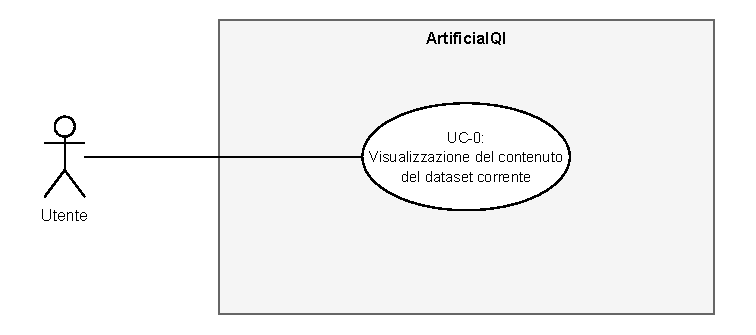
\includegraphics{Sezioni/UseCase/Immagini/UC-0.pdf}
    \caption{Diagramma UC-0.}
\end{figure}

\begin{usecase}{UC-0}{Visualizzazione di un dataset}
    
    \req{\hyperref[item:RU-1]{RU-1}} 

    \pre{
        \item Il sistema è attivo e funzionante
        \item Il dataset esiste
    }

    \post{
        \item Viene visualizzato il dataset
    }
    
    \actor{Utente}

    \subactors{}

    \trigger{L'utente deve visualizzare il dataset}
    
    \inc{}

    \base{}

    \scenario{
        \item L'utente richiede la visualizzazione del dataset
        \item Le coppie del dataset vengono mostrate in una lista
    }

    \subscenario{
        \item[2.1] \textbf{Il dataset è vuoto}
        \begin{itemize}
            \item[a.] Viene indicato all'utente che il dataset è vuoto
        \end{itemize}
    }
\end{usecase}

\subsection{UC-1}
\begin{figure}[H]
    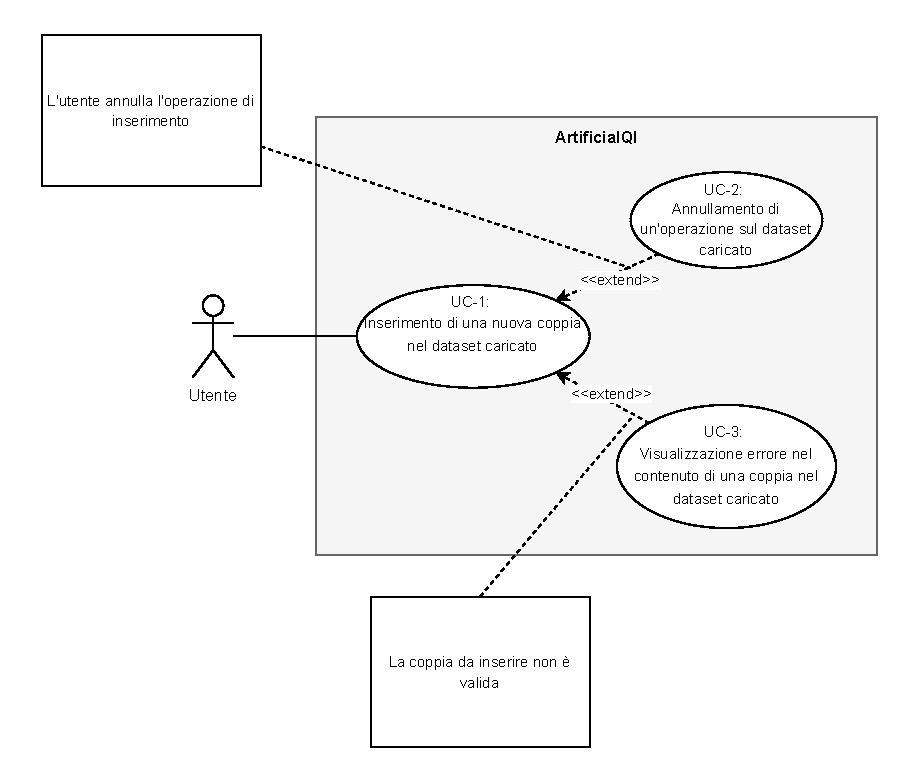
\includegraphics[scale=0.8]{Sezioni/UseCase/Immagini/UC-1.pdf}
    \caption{Diagramma UC-1.}
\end{figure}


\begin{usecase}{UC-1}{Inserimento di una nuova coppia nel dataset corrente}
    
    \req{\hyperref[item:RU-1]{RU-1}} 

    \pre{
        \item Il sistema è attivo e funzionante
    }

    \post{
        \item Viene inserita una nuova coppia nel dataset corrente
    }
    
    \actor{Utente}

    \subactors{}

    \trigger{L'utente vuole inserire di una nuova coppia nel dataset corrente}
    
    \inc{}

    \base{}

    \scenario{
        \item L'utente richiede l'inserimento di una nuova coppia
        \item L'utente specifica il contenuto per la nuova coppia
        \item L'utente conferma l'inserimento della nuova coppia
        \item La coppia viene inserita nel dataset corrente
    }

    \subscenario{
        \item[2.1] \textbf{L'utente annulla l'operazione di inserimento} 
        \begin{itemize}
            \item[a.] \hyperref[subsec:UC-2]{UC-2}
        \end{itemize}
        \item[3.1] \textbf{La coppia da inserire non è valida}
        \begin{itemize}
            \item[a.] \hyperref[subsec:UC-3]{UC-3}
        \end{itemize}
    }
\end{usecase}




\subsection{UC-2}
\label{subsec:UC-2}
\begin{usecase}{UC-2}{Annullamento di un'operazione sul dataset caricato}

        \req{}
        
        \pre{
            \item Il sistema è attivo e funzionante     
            \item L'utente è coinvolto in un'operazione di modifica del dataset caricato
        }
        
        \post{ 
            \item L'operazione viene interrotta 
            \item Il dataset caricato resta invariato
        }

        \actor{Utente}
        
        \subactors{}
        
        \trigger{L'utente richiede l'annullamento dell'operazione}
        
        \inc{}
        
        \base{}
        
        \scenario{
            \item L'utente richiede l'annullamento dell'operazione sul dataset caricato 
            \item La modifica al dataset caricato viene annullata 
            \item Il dataset caricato resta invariato 
        }
        
        
\end{usecase}

\subsection{UC-3}
\label{subsec:UC-3}

\begin{usecase}{UC-3}{Visualizzazione errore nel contenuto di una coppia del dataset corrente}
            
    \req{}
    
    \pre{
        \item Il sistema è attivo e funzionante
        \item Sia la domanda che la risposta della coppia sono vuote
    }
    
    \post {
        \item Viene richiesta la correzione della coppia
    }
    
    \actor{Utente}
    
    \subactors{}

    \trigger{Una coppia è invalida}
    
    \inc{}
    
    \base{}
    
    \scenario{
        \item Viene visualizzato un messaggio di errore che richiede la corretta compilazione di almeno una tra domanda e risposta
    }
\end{usecase}


\subsection{UC-4}

\begin{figure}[H]
    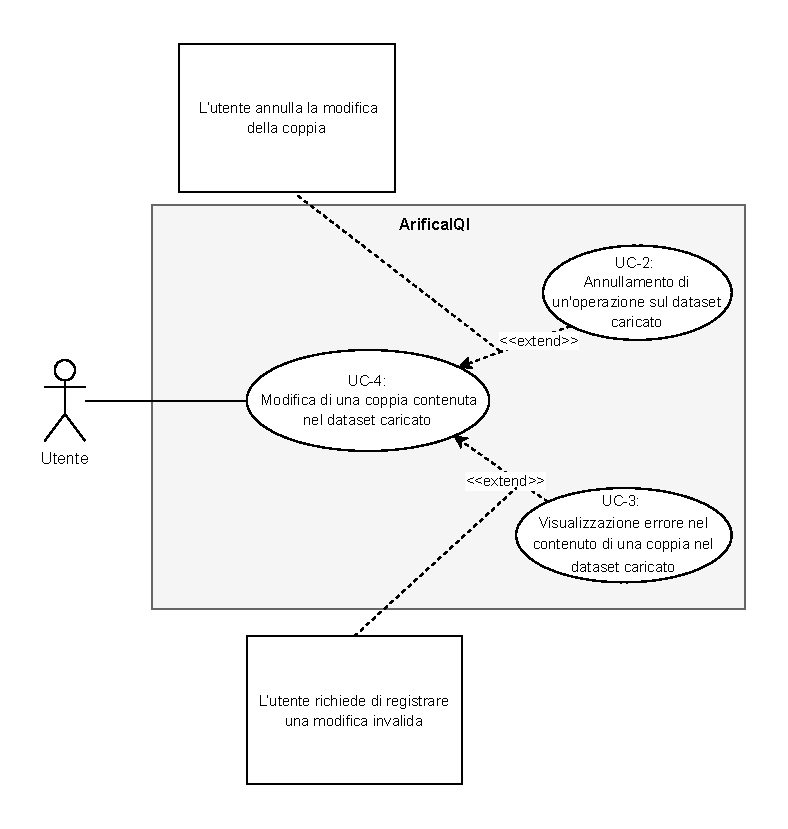
\includegraphics[scale=0.8]{Sezioni/UseCase/Immagini/UC-4.pdf}
    \caption{Diagramma UC-4.}
\end{figure}

\begin{usecase}{UC-4}{Modifica di una coppia contenuta nel dataset corrente}
    
    \req{\hyperref[item:RU-1]{RU-1}} 

    \pre{
        \item Il sistema è attivo e funzionante
        \item Il dataset corrente non è vuoto
        \item La coppia da modificare esiste
    }

    \post{
        \item La coppia viene aggiornata
        \item Il dataset corrente viene aggiornato
    }
    
    \actor{Utente}

    \subactors{}

    \trigger{L'utente deve modificare una coppia contenuta nel dataset corrente}
    
    \inc{}

    \base{}

    \scenario{
        \item L'utente richiede la modifica di una coppia
        \item L'utente modifica il contenuto della coppia
        \item L'utente conferma la modifica della coppia
        \item La coppia viene aggiornata nel dataset corrente

    }

    \subscenario{
        \item[2.1] \textbf{L'utente annulla la modifica della coppia} 
        \begin{itemize}
            \item[a.] \hyperref[subsec:UC-2]{UC-2}
        \end{itemize}
        \item[3.1] \textbf{L'utente richiede di registrare una modifica invalida}
        \begin{itemize}
            \item[a.] \hyperref[subsec:UC-3]{UC-3}
        \end{itemize}
    }
\end{usecase}


\subsection{UC-5}

\begin{figure}[H]
    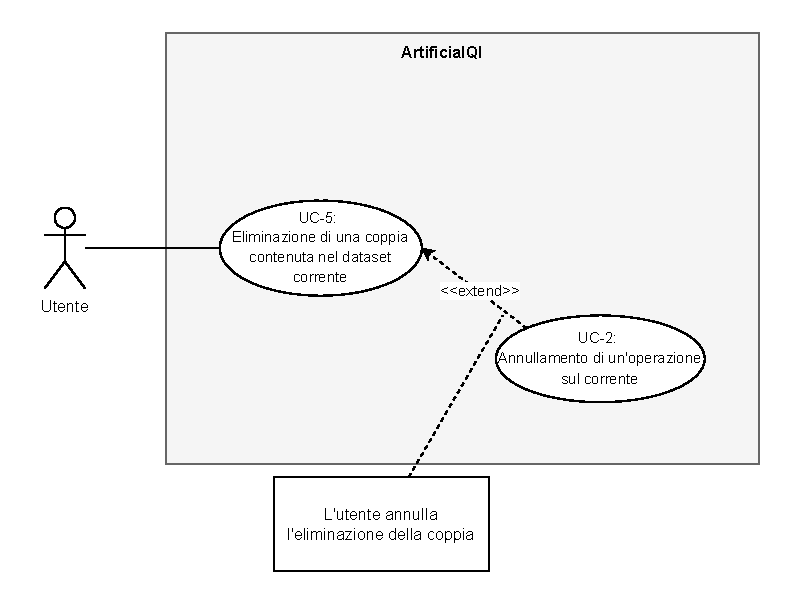
\includegraphics{Sezioni/UseCase/Immagini/UC-5.pdf}
    \caption{Diagramma UC-5.}
\end{figure}

\begin{usecase}{UC-5}{Eliminazione di una coppia contenuta nel dataset corrente}
    
    \req{\hyperref[item:RU-1]{RU-1}} 

    \pre{
        \item Il sistema è attivo e funzionante
        \item Il dataset corrente non è vuoto
        \item La coppia da eliminare esiste
    }

    \post{
        \item La coppia viene eliminata dal dataset corrente
    }
    
    \actor{Utente}

    \subactors{}

    \trigger{L'utente deve eliminare una coppia contenuta nel dataset corrente}
    
    \inc{}

    \base{}

    \scenario{
        \item L'utente richiede l'eliminazione della coppia
        \item L'utente conferma l'eliminazione
        \item La coppia viene eliminata dal dataset corrente
    }

    \subscenario{
        \item[2.1] \textbf{L'utente annulla l'eliminazione della coppia:} 
        \begin{itemize}
            \item[a.] \hyperref[subsec:UC-2]{UC-2}
        \end{itemize}
    }
\end{usecase}


\subsection{UC-6}

\begin{figure}[H]
    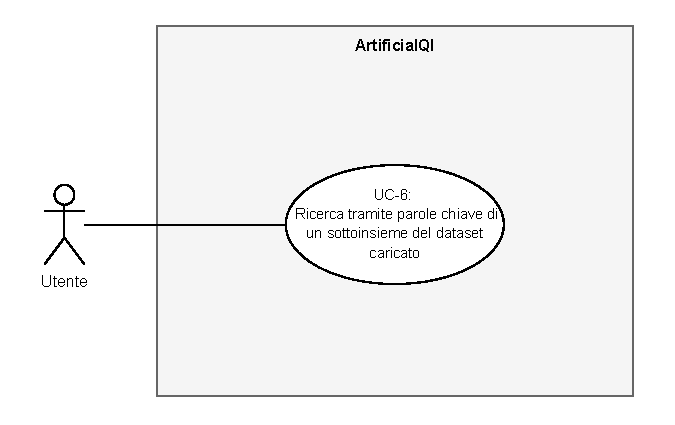
\includegraphics{Sezioni/UseCase/Immagini/UC-6.pdf}
    \caption{Diagramma UC-6.}
\end{figure}

\begin{usecase}{UC-6}{Ricerca tramite parole chiave di un sottoinsieme del dataset corrente}
    
    \req{\hyperref[item:RU-2]{RU-2}} 

    \pre{
        \item Il sistema è attivo e funzionante
        \item Il dataset su cui effettuare la ricerca è stato caricato come dataset corrente
        \item Il dataset corrente non è vuoto
    }

    \post{
        \item Viene mostrato il sottoinsieme del dataset corrente risultante dall'operazione di ricerca
    }
    
    \actor{Utente}

    \subactors{}

    \trigger{L'utente deve cercare una o più coppie contenute nel dataset corrente}
    
    \inc{}

    \base{}

    \scenario{
        \item L'utente specifica le parole chiave
        \item L'utente conferma l'esecuzione della ricerca
        \item Viene mostrata la lista di coppie che contengono le parole chiave nella domanda e/o nella risposta
    }

    \subscenario{
        \item[1.1] \textbf{Non vengono indicate parole chiave}
        \begin{itemize}
            \item [a.] L'utente conferma l'esecuzione della ricerca
            \item [b.] Viene mostrato l'intero dataset corrente
        \end{itemize}
        \item[3.1]\textbf{Il sottoinsieme risultante è vuoto}
        \begin{itemize}
            \item[a.] Viene notificato all'utente che la ricerca non ha prodotto risultati
        \end{itemize}
    }
\end{usecase}


\subsection{UC-7}

\begin{figure}[H]
    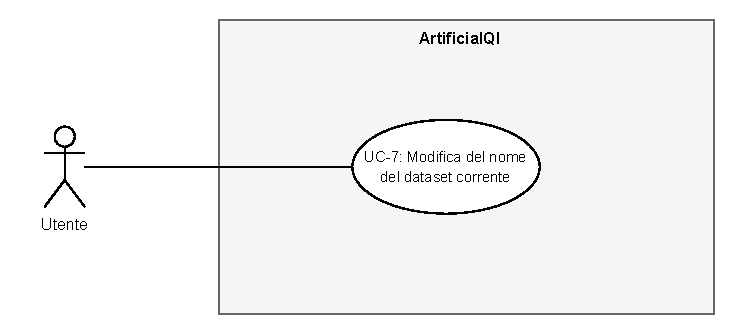
\includegraphics{Sezioni/UseCase/Immagini/UC-7.pdf}
    \caption{Diagramma UC-7.}
\end{figure}

\begin{usecase}{UC-7}{Modifica del nome di un dataset }
    
    \req{\hyperref[item:RU-1]{RU-1}} 

    \pre{
        \item Il sistema è attivo e funzionante
        \item Il dataset da rinominare esiste
    }

    \post{
        \item Il dataset viene rinominato
    }
    
    \actor{Utente}

    \subactors{}

    \trigger{L'utente vuole modificare il nome di un dataset }
    
    \inc{}

    \base{}

    \scenario{
        \item L'utente richiede la modifica del nome di un dataset 
        \item L'utente specifica il nuovo nome
        \item L'utente conferma la modifica 
        \item Il dataset viene rinominato
    }

    \subscenario{
        \item[2.1] \textbf{L'utente annulla l'operazione di modifica}
        \begin{itemize}
            \item [a.] Il nome del dataset resta invariato
            \item [b.] L'operazione di modifica viene terminata
        \end{itemize}
        \item[3.1] \textbf{Il nuovo nome del dataset è vuoto o già esiste}
        \begin{itemize}
            \item [a.] \hyperref[subsec:UC-8]{UC-8}
        \end{itemize}
    }
\end{usecase}

\subsection{UC-8}
\label{subsec:UC-8}

\begin{usecase}{UC-8}{Visualizzazione errore nel nome di un dataset}
    
    \req{} 

    \pre{
        \item Il sistema è attivo e funzionante
        \item Il nome del dataset è invalido
    }

    \post{
        \item Viene richiesto all'utente di fornire un nome valido
    }
    
    \actor{Utente}

    \subactors{}

    \trigger{Il nome del dataset è invalido}
    
    \inc{}

    \base{}

    \scenario{
        \item Viene visualizzato un messaggio di errore che richiede
        la corretta compilazione del nome del dataset
    }
\end{usecase}

\subsection{UC-9}
\label{subsec:UC-9}


\begin{figure}[H]
    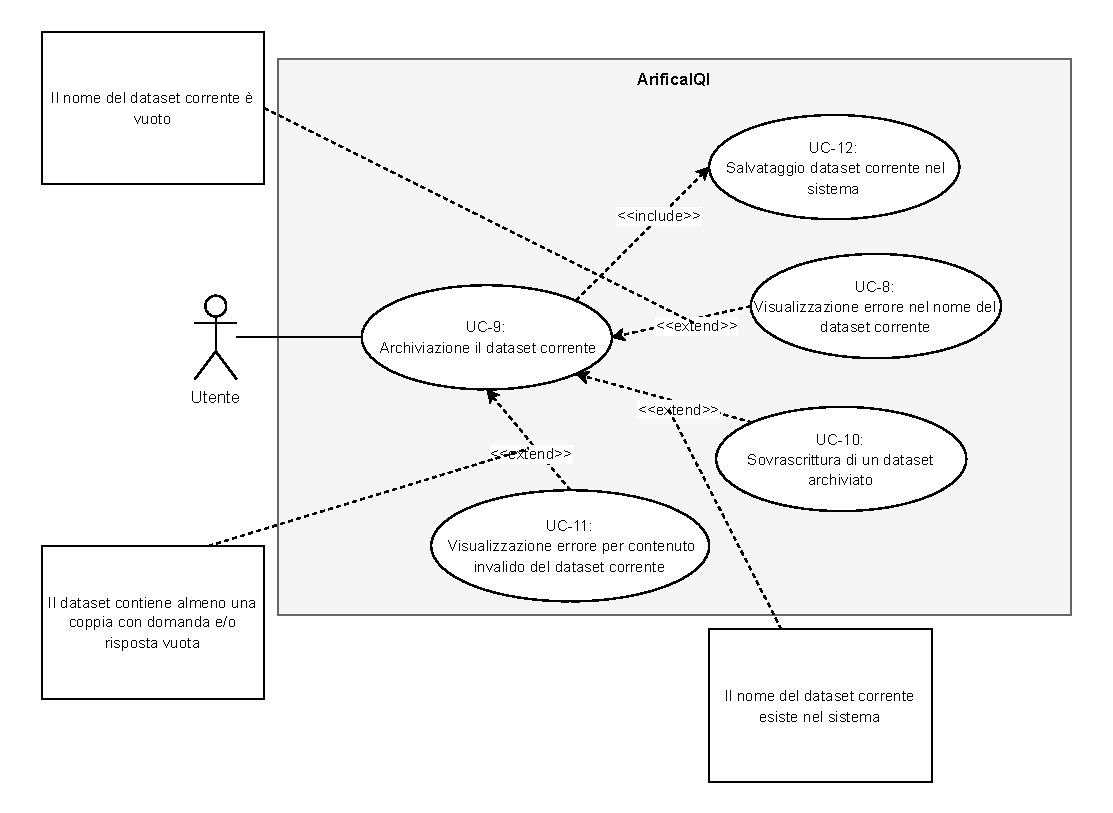
\includegraphics[scale=0.75]{Sezioni/UseCase/Immagini/UC-9.pdf}
    \caption{Diagramma UC-9.}
\end{figure}

\begin{usecase}{UC-9}{Archiviazione del dataset corrente}
    
    \req{\hyperref[item:RU-3]{RU-3}} 

    \pre{
        \item Il sistema è attivo e funzionante
        \item Il dataset corrente non è vuoto
    }

    \post{
        \item Il dataset corrente viene archiviato nel sistema
    }
    
    \actor{Utente}

    \subactors{}

    \trigger{L'utente deve archiviare il dataset corrente per renderlo persistente}
    
    \inc{\hyperref[subsec:UC-12]{UC-12}}

    \base{}

    \scenario{
        \item L'utente richiede l'archiviazione del dataset corrente.
        \item \texttt{<<include:UC-12>>}
    }

    \subscenario{
        \item[1.1] \textbf{Il nome del dataset corrente è vuoto}
        \begin{itemize}
            \item [a.] \hyperref[subsec:UC-8]{UC-8}
        \end{itemize}
        \item[1.2]\textbf{Esiste già un dataset archiviato nel sistema con nome uguale al dataset corrente}
        \begin{itemize}
            \item[a.] \hyperref[subsec:UC-10]{UC-10}
        \end{itemize}
        \item[1.3] \textbf{Il dataset contiene almeno una coppia con domanda e/o risposta vuota}
        \begin{itemize}
            \item[a.] \hyperref[subsec:UC-11]{UC-11}
        \end{itemize}
    }
\end{usecase}


\subsection{UC-10}
\label{subsec:UC-10}

\begin{usecase}{UC-10}{Sovrascrittura di un dataset archiviato}
    \req{\hyperref[item:RU-3]{RU-3}} 

    \pre{
        \item Il sistema è attivo e funzionante
        \item Il dataset corrente possiede già una versione archiviata
    }

    \post{
        \item La versione archiviata del dataset corrente viene sovrascritta
    }
    
    \actor{Utente}

    \subactors{}

    \trigger{L'utente deve aggiornare la versione archiviata di un dataset}
    
    \inc{\hyperref[subsec:UC-12]{UC-12}}

    \base{}

    \scenario{
        \item L'utente richiede l'archiviazione del dataset corrente che possiede già una versione archiviata.
        \item L'utente conferma la sovrascrittura
        \item \texttt{<<include:UC-12>>}
    }

    \subscenario{
        \item[2.1] \textbf{L'utente non conferma la sovrascrittura}
        \begin{itemize}
            \item [a.] L'operazione di sovrascrittura viene interrotta
        \end{itemize}
    }
\end{usecase}

\subsection{UC-11}
\label{subsec:UC-11}

\begin{usecase}{UC-11}{Visualizzazione errore per contenuto invalido del dataset corrente}
    \req{} 

    \pre{
        \item Il sistema è attivo e funzionante
        \item Il dataset corrente contiene almeno una coppia invalida ovvero avente domanda e/o risposta vuota
    }

    \post{
        \item L'utente conosce le coppie invalide contenute nel dataset corrente
    }
    
    \actor{Utente}

    \subactors{}

    \trigger{Il dataset corrente contiene almeno una coppia invalida}
    
    \inc{}

    \base{}

    \scenario{
        \item Viene notificata all'utente la presenza di coppie invalide
        \item Vengono evidenziate le coppie invalide
    }
\end{usecase}

\subsection{UC-12}
\label{subsec:UC-12}

\begin{figure}[H]
    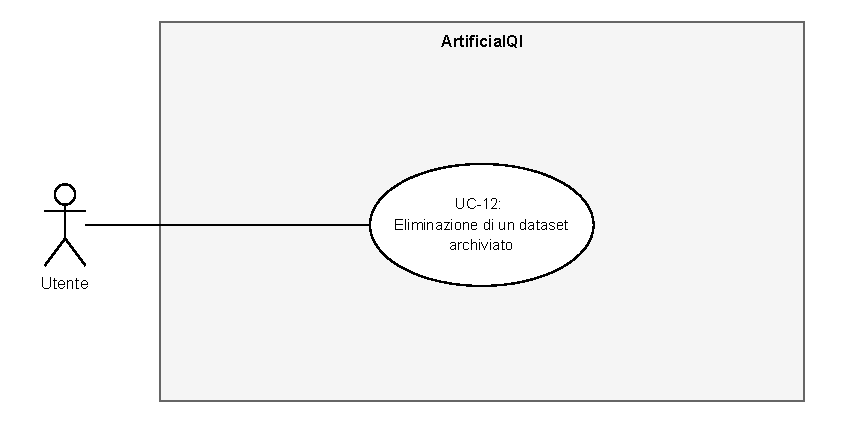
\includegraphics{Sezioni/UseCase/Immagini/UC-12.pdf}
    \caption{Diagramma UC-12.}
\end{figure}

\begin{usecase}{UC-12}{Eliminazione di un dataset archiviato}

    \req{\hyperref[item:RU-3]{RU-3}} 

    \pre{
        \item Il sistema è attivo e funzionante
        \item Il dataset archiviato da eliminare esiste
    }

    \post{
        \item Il dataset selezionato viene eliminato 
    }
    
    \actor{Utente}

    \subactors{}

    \trigger{L'utente deve eliminare un dataset archiviato}
    
    \inc{}

    \base{}

    \scenario{
        \item L'utente richiede l'eliminazione di un dataset archiviato
        \item L'utente conferma l'eliminazione del dataset selezionato
        \item Il dataset viene eliminato dal sistema
    }

    \subscenario{
        \item[2.1] \textbf{L'utente annulla l'eliminazione del dataset selezionato}
        \begin{itemize}
            \item[a.] Il dataset selezionato non viene eliminato
            \item[b.] Viene interrotta l'operazione di eliminazione
        \end{itemize}
        \item[3.1] \textbf{L'eliminazione del dataset dal sistema produce un errore}
        \begin{itemize}
        \item[a.] Viene notificato all'utente l'errore che ha impedito la corretta eliminazione del dataset selezionato
        \end{itemize}
    }

\end{usecase}

\subsection{UC-13}
\label{subsec:UC-13}

\begin{figure}[H]
    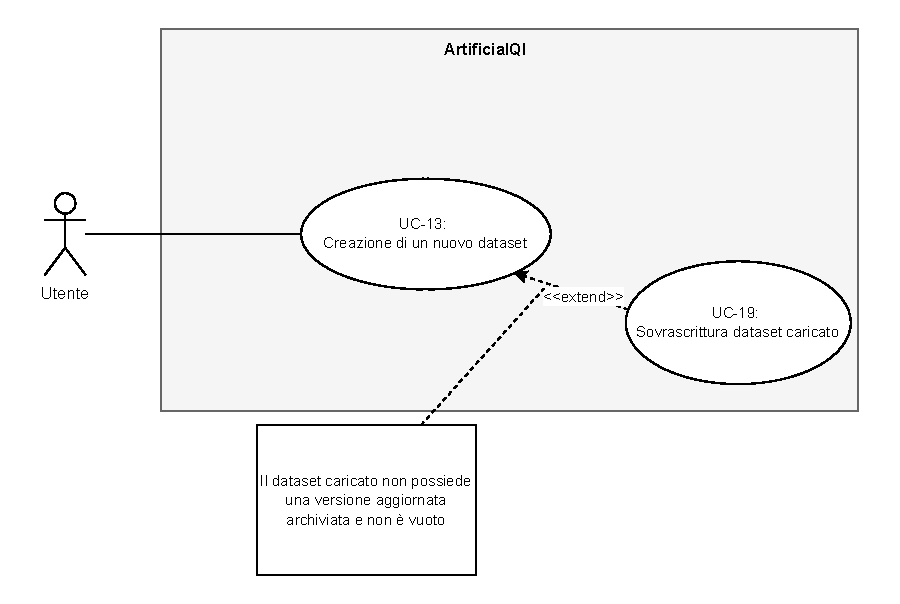
\includegraphics{Sezioni/UseCase/Immagini/UC-13.pdf}
    \caption{Diagramma UC-13.}
\end{figure}

\begin{usecase}{UC-13}{Creazione di un nuovo dataset}

    \req{\hyperref[item:RU-3]{RU-3}} 

    \pre{
        \item Il sistema è attivo e funzionante
    }

    \post{
        \item Il nuovo dataset temporaneo viene caricato
    }
    
    \actor{Utente}

    \subactors{}

    \trigger{L'utente deve creare un nuovo dataset}
    
    \inc{}

    \base{}

    \scenario{
        \item L'utente richiede la creazione di un nuovo dataset
        \item Viene creato un nuovo dataset temporaneo vuoto
        \item Il dataset temporaneo viene caricato
    }

    \subscenario{
        \item[2.1] \textbf{Il dataset caricato non possiede una versione aggiornata archiviata e non è vuoto}
        \begin{itemize}
            \item[a.] \hyperref[subsec:UC-19]{UC-19}
        \end{itemize}
    }

\end{usecase}

\subsection{UC-14}
\label{subsec:UC-14}

\begin{figure}[H]
    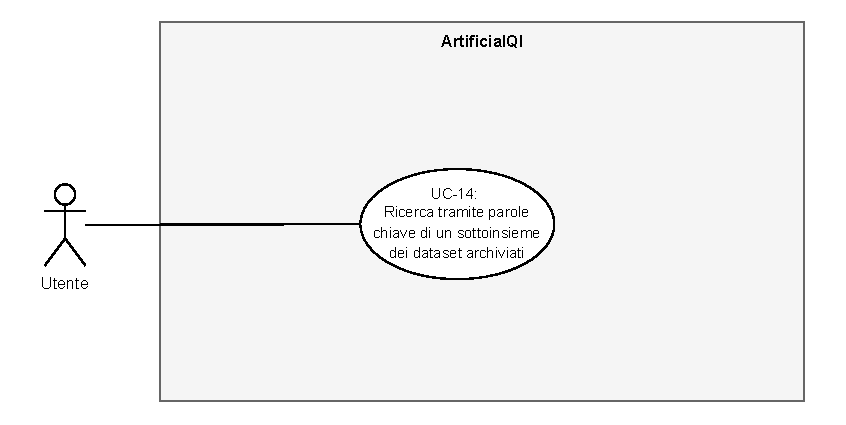
\includegraphics{Sezioni/UseCase/Immagini/UC-14.pdf}
    \caption{Diagramma UC-14.}
\end{figure}

\begin{usecase}{UC-14}{Caricamento di un dataset archiviato}

    \req{\hyperref[item:RU-4]{RU-4}} 

    \pre{
        \item Il sistema è attivo e funzionante
        \item Il dataset da caricare è stato precedentemente archiviato
    }

    \post{
        \item Il dataset viene caricato
    }
    
    \actor{Utente}

    \subactors{}

    \trigger{L'utente deve caricare un dataset tra quelli archiviati nel sistema}
    
    \inc{}

    \base{}

    \scenario{
        \item L'utente richiede di caricare un dataset archiviato nel sistema
        \item L'utente seleziona il nome del dataset tra quelli archiviati
        \item Il dataset scelto viene caricato
    }

    \subscenario{
        \item[3.1] \textbf{Il dataset caricato non possiede una versione aggiornata archiviata e non è vuoto}
        \begin{itemize}
            \item[a.] \hyperref[subsec:UC-15]{UC-15}
        \end{itemize}
    }
\end{usecase}

\subsection{UC-15}
\label{subsec:UC-15}


\begin{figure}[H]
    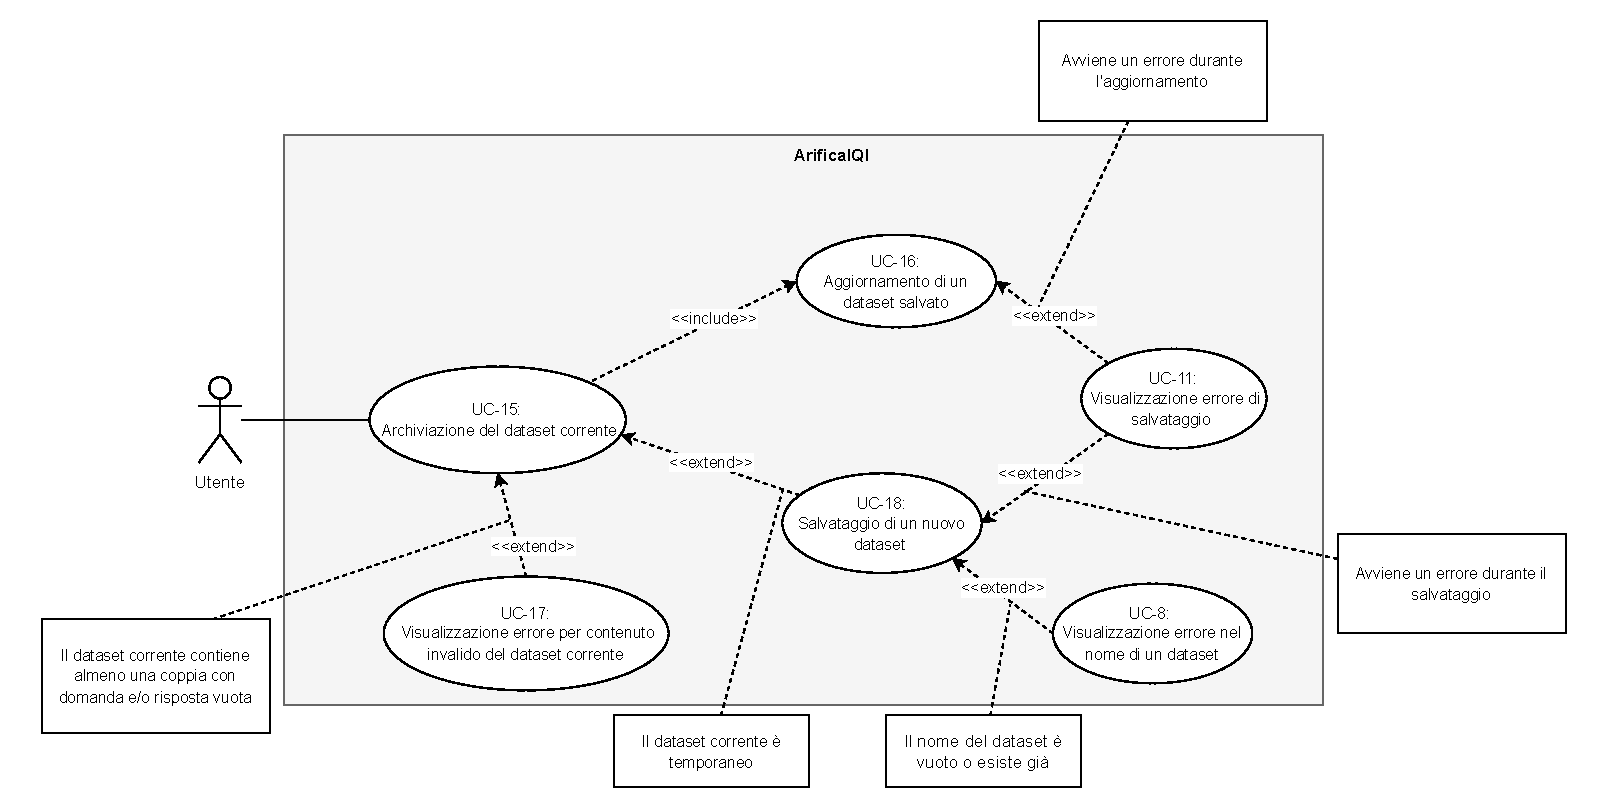
\includegraphics[scale=0.60]{Sezioni/UseCase/Immagini/UC-15.pdf}
    \caption{Diagramma UC-15.}
\end{figure}

\begin{usecase}{UC-15}{Archiviazione del dataset corrente}
    
    \req{\hyperref[item:RU-5]{RU-5}} 

    \pre{
        \item Il sistema è attivo e funzionante
        \item Il dataset da archiviare è stato caricato come dataset corrente
        \item Il dataset corrente non è vuoto
        \item Il dataset corrente non possiede una copia archiviata aggiornata
    }

    \post{
        \item Il dataset corrente viene archiviato nel sistema
    }
    
    \actor{Utente}

    \subactors{}

    \trigger{L'utente deve archiviare il dataset corrente per renderlo persistente}
    
    \inc{\hyperref[subsec:UC-16]{UC-16}}

    \base{}

    \scenario{
        \item L'utente richiede l'archiviazione del dataset corrente.
        \item \texttt{<<include:UC-16>>}
    }

    \subscenario{
        \item[1.1] \textbf{Il dataset corrente contiene almeno una coppia con domanda e/o risposta vuota}
        \begin{itemize}
            \item[a.] \hyperref[subsec:UC-17]{UC-17}
        \end{itemize}
        \item[1.2] \textbf{Il dataset corrente è temporaneo perchè è stato appena creato}
        \begin{itemize}
            \item[a.] \hyperref[subsec:UC-18]{UC-18}
        \end{itemize}
    }
\end{usecase}


\subsection{UC-16}
\label{subsec:UC-16}

\begin{usecase}{UC-16}{Salvataggio del dataset caricato nel sistema}
    \req{} 

    \pre{
        \item Il sistema è attivo e funzionante
    }

    \post{
        \item Il dataset caricato viene salvato nel sistema
        \item L'utente è a conoscenza del corretto salvataggio
    }
    
    \actor{Utente}

    \subactors{}

    \trigger{Il sistema deve salvare il dataset caricato}
    
    \inc{}

    \base{}

    \scenario{
        \item Il dataset caricato viene salvato nel sistema
    }

    \subscenario{
        \item[1.1] \textbf{Avviene un errore durante il salvataggio del dataset caricato}
        \begin{itemize}
            \item[a.] \hyperref[subsec:UC-11]{UC-11}
        \end{itemize}
    }

\end{usecase}

\subsection{UC-17}
\label{subsec:UC-17}

\begin{figure}[H]
    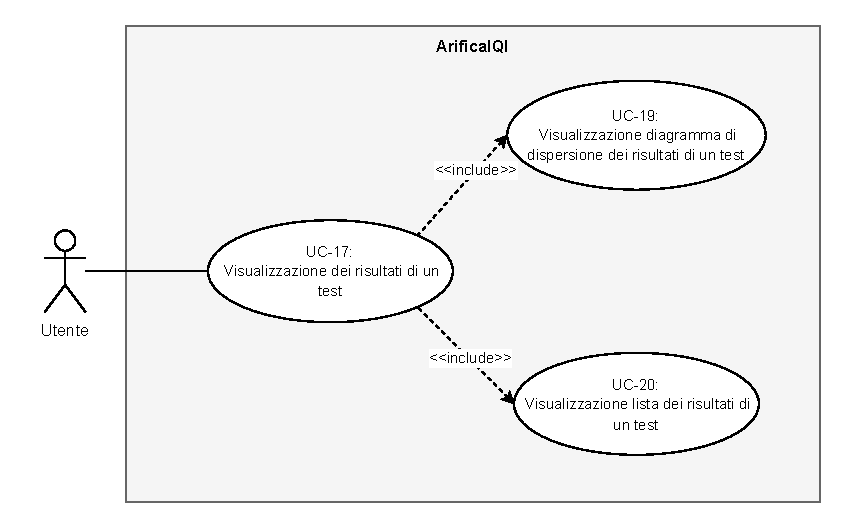
\includegraphics{Sezioni/UseCase/Immagini/UC-17.pdf}
    \caption{Diagramma UC-17.}
\end{figure}

\begin{usecase}{UC-17}{Visualizzazione dei risultati di un test}

    \req{\hyperref[item:RU-6]{RU-6}} 

    \pre{
        \item Il sistema è attivo e funzionante
        \item Sono disponibili i risultati di un test
    }

    \post{
        \item L'utente conosce l'esito del test
    }
    
    \actor{Utente}

    \subactors{}

    \trigger{L'utente deve testare il LLM usando il dataset corrente}
    
    \inc{\hyperref[subsec:UC-19]{UC-19}, \hyperref[subsec:UC-20]{UC-20}}

    \base{}

    \scenario{
        \item \texttt{<<include:UC-19>>}
        \item \texttt{<<include:UC-20>>}
    }

\end{usecase}

\subsection{UC-18}
\label{subsec:UC-18}

\begin{figure}[H]
    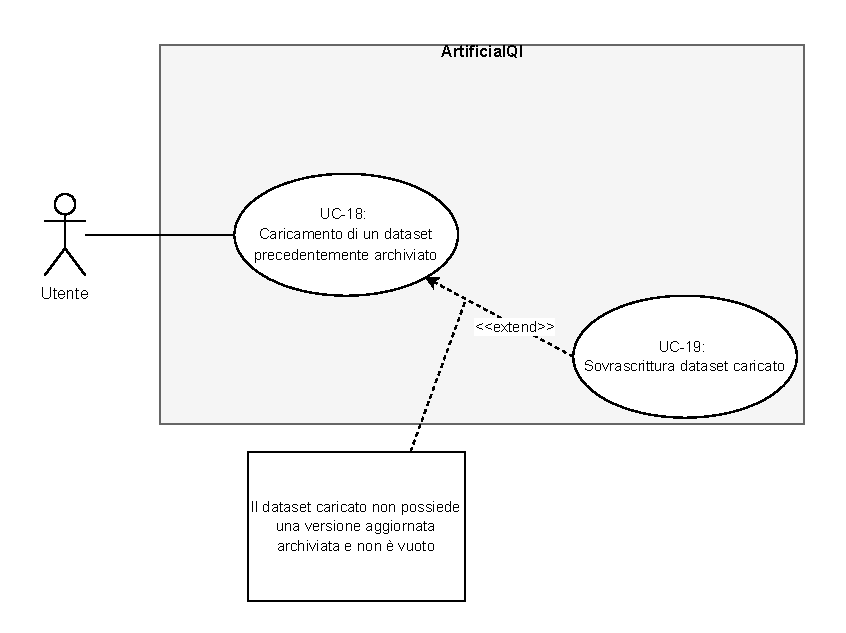
\includegraphics{Sezioni/UseCase/Immagini/UC-18.pdf}
    \caption{Diagramma UC-18.}
\end{figure}

\begin{usecase}{UC-18}{Caricamento di un dataset archiviato}

    \req{\hyperref[item:RU-6]{RU-6}} 

    \pre{
        \item Il sistema è attivo e funzionante
        \item Il dataset da caricare è stato precedentemente archiviato
    }

    \post{
        \item Il dataset viene caricato
    }
    
    \actor{Utente}

    \subactors{}

    \trigger{L'utente deve caricare un dataset tra quelli archiviati nel sistema}
    
    \inc{}

    \base{}

    \scenario{
        \item L'utente richiede di caricare un dataset archiviato nel sistema
        \item L'utente seleziona il nome del dataset tra quelli archiviati
        \item Il dataset scelto viene caricato
    }

    \subscenario{
        \item[3.1] \textbf{Il dataset caricato non possiede una versione aggiornata archiviata e non è vuoto}
        \begin{itemize}
            \item[a.] \hyperref[subsec:UC-19]{UC-19}
        \end{itemize}
    }
\end{usecase}

\subsection{UC-19}
\label{subsec:UC-19}

\begin{figure}[H]
    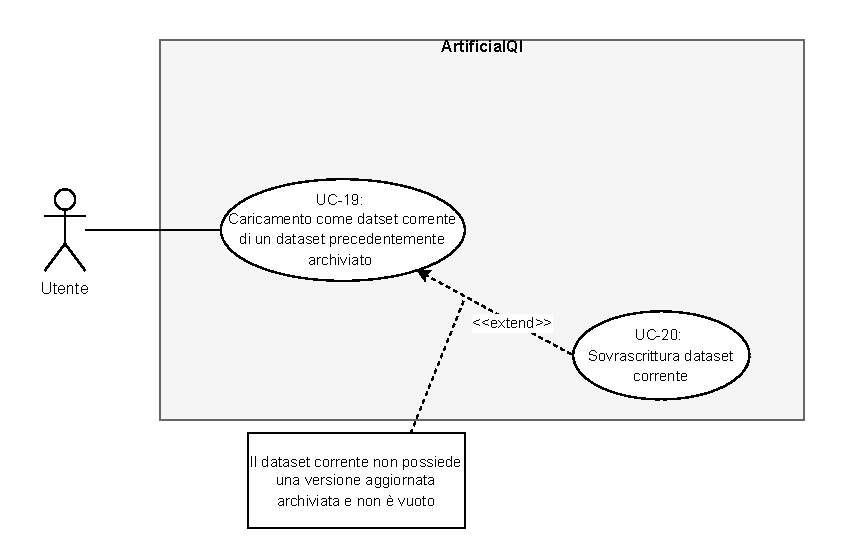
\includegraphics{Sezioni/UseCase/Immagini/UC-19.pdf}
    \caption{Diagramma UC-19.}
\end{figure}

\begin{usecase}{UC-19}{Caricamento come dataset corrente di un dataset archiviato}

    \req{\hyperref[item:RU-6]{RU-6}} 

    \pre{
        \item Il sistema è attivo e funzionante
        \item Il dataset da caricare come dataset corrente è stato precedentemente archiviato
    }

    \post{
        \item Il dataset viene caricato come dataset corrente
    }
    
    \actor{Utente}

    \subactors{}

    \trigger{L'utente deve caricare come dataset corrente uno tra quelli archiviati}
    
    \inc{}

    \base{}

    \scenario{
        \item L'utente richiede di caricare un dataset archiviato
        \item L'utente seleziona il nome del dataset tra quelli archiviati
        \item Il dataset scelto viene caricato come dataset corrente
    }

    \subscenario{
        \item[3.1] \textbf{Il dataset caricato non possiede una versione aggiornata archiviata e non è vuoto}
        \begin{itemize}
            \item[a.] \hyperref[subsec:UC-20]{UC-20}
        \end{itemize}
    }
\end{usecase}

\subsection{UC-20}
\label{subsec:UC-20}

\begin{usecase}{UC-20}{Visualizzazione lista dei risultati di un test}

    \req{\hyperref[item:RU-6]{RU-6}} 

    \pre{
        \item Il sistema è attivo e funzionante
        \item È stato eseguito correttamente il test sul dataset caricato
    }

    \post{
        \item L'utente visualizza la lista dei risultati del test
    }
    
    \actor{Utente}

    \subactors{LLM}

    \trigger{}
    
    \inc{}

    \base{}

    \scenario{
        \item Viene mostrata la lista dei risultati del test.
        
        
        \item Ogni elemento è composto da: domanda, risposta attesa, risposta ottenuta dal LLM, grado di somiglianza tra le due risposte e valutazione di correttezza della risposta.
    }

\end{usecase}

\subsection{UC-21}
\label{subsec:UC-21}

\begin{usecase}{UC-21}{Visualizzazione errore di comunicazione con LLM}

    \req{} 

    \pre{
        \item Il sistema è attivo e funzionante
        \item La comunicazione con il LLM non è andata a buon fine
    }

    \post{
        \item L'utente conosce l'errore di comunicazione
    }
    
    \actor{Utente}

    \subactors{LLM}

    \trigger{La comunicazione con il LLM produce un errore}
    
    \inc{}

    \base{}

    \scenario{
        \item Viene mostrato un messaggio di errore all'utente
    }

\end{usecase}

\subsection{UC-22}
\label{subsec:UC-22}

\begin{usecase}{UC-22}{Eliminazione di un dataset archiviato}

    \req{\hyperref[item:RU-6]{RU-6}} 

    \pre{
        \item Il sistema è attivo e funzionante
        \item Il dataset archiviato da eliminare esiste
    }

    \post{
        \item Il dataset selezionato viene eliminato 
    }
    
    \actor{Utente}

    \subactors{}

    \trigger{L'utente deve eliminare un dataset archiviato}
    
    \inc{}

    \base{}

    \scenario{
        \item L'utente richiede l'eliminazione di un dataset archiviato
        \item L'utente conferma l'eliminazione del dataset selezionato
        \item Il dataset viene eliminato dal sistema
    }

    \subscenario{
        \item[2.1] \textbf{L'utente annulla l'eliminazione del dataset selezionato}
        \begin{itemize}
            \item[a.] Il dataset selezionato non viene eliminato
            \item[b.] Viene interrotta l'operazione di eliminazione
        \end{itemize}
        \item[3.1] \textbf{L'eliminazione del dataset dal sistema produce un errore}
        \begin{itemize}
        \item[a.] Viene notificato all'utente l'errore che ha impedito la corretta eliminazione del dataset selezionato
        \end{itemize}
    }

\end{usecase}

\subsection{UC-23}
\label{subsec:UC-23}

\begin{usecase}{UC-23}{Visualizzazione errore di salvataggio del dataset}
    \req{} 

    \pre{
        \item Il sistema è attivo e funzionante
    }

    \post{
        \item L'utente conosce la causa del errore di salvataggio
    }
    
    \actor{Utente}

    \subactors{}

    \trigger{Il sistema riscontra un errore nel salvataggio del dataset }
    
    \inc{}

    \base{}

    \scenario{
        \item Viene notificato all'utente l'errore che ha impedito il corretto salvataggio del dataset 
    }

\end{usecase}

\subsection{UC-24}
\label{subsec:UC-24}

\begin{usecase}{UC-24}{Visualizzazione diagramma di dispersione dei risultati di un test}

    \req{} 

    \pre{
        \item Il sistema è attivo e funzionante
        \item È stato eseguito correttamente il test sul dataset caricato
    }

    \post{
        \item L'utente visualizza un diagramma di dispersione
    }
    
    \actor{Utente}

    \subactors{LLM}

    \trigger{}
    
    \inc{}

    \base{}

    \scenario{
        \item Visualizzazione di un grafico di dispersione.
        L'asse delle ordinate rappresenta il numero della domanda.
        L'asse delle ascisse rappresenta il grado di somiglianza tra la risposta attesa e la risposta effettiva.
        
        \item Rappresentazione dei risultati come punti distinguibili tra risposta corretta e sbagliata.
        
        \item Calcolo della media e rappresentazione come una retta nel grafico.
        
        \item Calcolo della deviazione standard come una retta nel grafico.
        
        \item Mostrare la legenda del grafico.
    }

\end{usecase}

\subsection{UC-25}
\label{subsec:UC-25}

\begin{figure}[H]
    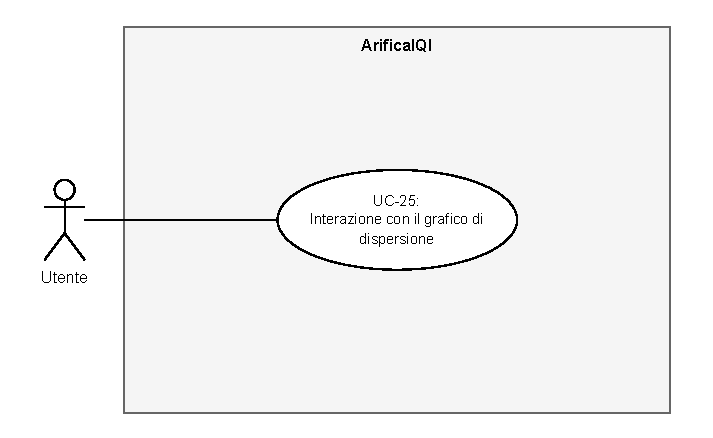
\includegraphics{Sezioni/UseCase/Immagini/UC-25.pdf}
    \caption{Diagramma UC-25.}
\end{figure}

\begin{usecase}{UC-25}{Interazione con il grafico di dispersione}

    \req{} 

    \pre{
        \item Il sistema è attivo e funzionante
        \item L'utente dispone del grafico di dispersione prodotto nella visualizzazione dei risultati del test
    }

    \post{
        \item Viene evidenziato il risultato relativo al punto del grafico di dispersione coinvolto nell'interazione.
    }
    
    \actor{Utente}

    \subactors{LLM}

    \trigger{L'utente ha la necessità di visualizzare un preciso risultato}
    
    \inc{}

    \base{}

    \scenario{
        \item L'utente interagisce con un punto del grafico di dispersione.
        
        
        \item Viene evidenziato l'elemento della lista dei risultati corrispondente al punto coinvolto nell'interazione.
    }

\end{usecase}